\documentclass[english]{beamer}\usepackage[]{graphicx}\usepackage[]{color}
%% maxwidth is the original width if it is less than linewidth
%% otherwise use linewidth (to make sure the graphics do not exceed the margin)
\makeatletter
\def\maxwidth{ %
  \ifdim\Gin@nat@width>\linewidth
    \linewidth
  \else
    \Gin@nat@width
  \fi
}
\makeatother

\definecolor{fgcolor}{rgb}{0.345, 0.345, 0.345}
\newcommand{\hlnum}[1]{\textcolor[rgb]{0.686,0.059,0.569}{#1}}%
\newcommand{\hlstr}[1]{\textcolor[rgb]{0.192,0.494,0.8}{#1}}%
\newcommand{\hlcom}[1]{\textcolor[rgb]{0.678,0.584,0.686}{\textit{#1}}}%
\newcommand{\hlopt}[1]{\textcolor[rgb]{0,0,0}{#1}}%
\newcommand{\hlstd}[1]{\textcolor[rgb]{0.345,0.345,0.345}{#1}}%
\newcommand{\hlkwa}[1]{\textcolor[rgb]{0.161,0.373,0.58}{\textbf{#1}}}%
\newcommand{\hlkwb}[1]{\textcolor[rgb]{0.69,0.353,0.396}{#1}}%
\newcommand{\hlkwc}[1]{\textcolor[rgb]{0.333,0.667,0.333}{#1}}%
\newcommand{\hlkwd}[1]{\textcolor[rgb]{0.737,0.353,0.396}{\textbf{#1}}}%
\let\hlipl\hlkwb

\usepackage{framed}
\makeatletter
\newenvironment{kframe}{%
 \def\at@end@of@kframe{}%
 \ifinner\ifhmode%
  \def\at@end@of@kframe{\end{minipage}}%
  \begin{minipage}{\columnwidth}%
 \fi\fi%
 \def\FrameCommand##1{\hskip\@totalleftmargin \hskip-\fboxsep
 \colorbox{shadecolor}{##1}\hskip-\fboxsep
     % There is no \\@totalrightmargin, so:
     \hskip-\linewidth \hskip-\@totalleftmargin \hskip\columnwidth}%
 \MakeFramed {\advance\hsize-\width
   \@totalleftmargin\z@ \linewidth\hsize
   \@setminipage}}%
 {\par\unskip\endMakeFramed%
 \at@end@of@kframe}
\makeatother

\definecolor{shadecolor}{rgb}{.97, .97, .97}
\definecolor{messagecolor}{rgb}{0, 0, 0}
\definecolor{warningcolor}{rgb}{1, 0, 1}
\definecolor{errorcolor}{rgb}{1, 0, 0}
\newenvironment{knitrout}{}{} % an empty environment to be redefined in TeX

\usepackage{alltt}

%% The most common packages are already included in:
\usetheme{biostat}
%%%%%%%%%%%%%%%%%%%%%%%%%%%%%%%%%%%%%%%%%%%%%%%%%%%%%%%% 
\usepackage{amsmath,amsfonts,tikz}
\usetikzlibrary{trees}

%% Header data: (adjust to your needs:
\def\uzhunit{Biostatistics}             %% if (not) needed comment/uncomment
%\def\uzhunitext{STA480}

\title{Publication Bias in the Cochrane Library of Systematic Reviews}
%% Optional Argument in [Brackets]: Short Title for Footline

%% The following are all optional, simply comment them
%\subtitle{Subtitle (optional)}
%\institute{Biostatistics Journal Club}  %% optional
\author{Giuachin Kreiliger}
%\date{\today}
%%%%%%%%%%%%%%%%%%%%%%%%%%%%%%%%%%%%%%%%%%%%%%%%%%%%%%%% 

%%%%%%%%%%%%%%%%%%%%%%%%%%%%%%%%%%%%%%%%%%%%%%%%%%%%%%%%
\IfFileExists{upquote.sty}{\usepackage{upquote}}{}
\begin{document}
\maketitle
%%%%%%%%%%%%%%%%%%%%%%%%%%%%%%%%%%%%%%%%%%%%%%%%%%%%%%%% 
%% Start with slides here: put them between `\begin{frame}` and `\end{frame}`


\begin{knitrout}
\definecolor{shadecolor}{rgb}{0.969, 0.969, 0.969}\color{fgcolor}\begin{kframe}


{\ttfamily\noindent\bfseries\color{errorcolor}{\#\# Error in UseMethod("{}mutate\_"{}): no applicable method for 'mutate\_' applied to an object of class "{}function"{}}}\end{kframe}
\end{knitrout}


\begin{frame}{Cochrane Library}
Database of high-quality, systematic reviews in clinical science.

Currently $\sim$ 8,000 reviews, prepared by independet groups. 

Reviews are peer-reviewed and prepared after guidelines.
\end{frame}


\begin{frame}{Cochrane Library Dataset}
5016 systematic reviews with studies published until 2018.

52995 studies.

463820 study results.
\end{frame}


\begin{frame}{Dataset structure}

\begin{figure}
\tikzstyle{every node}=[draw=black,thick,anchor=west,scale=.65]
\tikzstyle{selected}=[draw=red,fill=red!30]
\tikzstyle{optional}=[dashed,fill=gray!50]
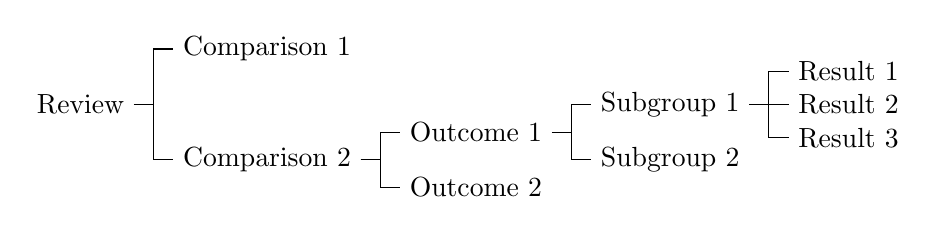
\begin{tikzpicture}
[grow = right, anchor = west, 
  growth parent anchor=east, % added code
  parent anchor=east, level distance=.5cm,
  sibling distance=2em, level 1/.style={sibling distance=2em}, level 2/.style={sibling distance=2em}, 
  level 3/.style={sibling distance=2em}, level 4/.style={sibling distance=1.2em}]
  \node {Review} [edge from parent fork right]
    child { node {Comparison 2}
      child { node {Outcome 2}}
      child { node {Outcome 1}
        child { node {Subgroup 2}}
        child { node {Subgroup 1}
          child  { node {Result 3}}
          child  { node {Result 2}}
          child  { node {Result 1}}
          }}
    }
    child [missing] {}		
    child { node {Comparison 1  }};
\end{tikzpicture}
%\caption{Structure of a hypothetical review with two different comparisons\label{review.structure}}
\label{review.structure}
\end{figure}

\end{frame}

\begin{frame}{Review Example}
\vspace{-5mm}
% latex table generated in R 3.5.1 by xtable 1.8-3 package
% Sun Apr 28 12:26:53 2019
\begin{table}[ht]
\centering
\begingroup\tiny
\begin{tabular}{lll}
  \hline
Study & Comparison & Outcome \\ 
  \hline
Bohn 1989 & Barbiturate vs no barbiturate & Death at the end of follow-up \\ 
  Bohn 1989 & Barbiturate vs no barbiturate & Death or severe disability at the end of follow-up \\ 
  Eisenberg 1988 & Barbiturate vs no barbiturate & Uncontrolled ICP during treatment \\ 
  Eisenberg 1988 & Barbiturate vs no barbiturate & Hypotension during treatment \\ 
  Perez-Barcena 2008 & Pentobarbital vs Thiopental & Death at the end of follow-up (6 months) \\ 
  Perez-Barcena 2008 & Pentobarbital vs Thiopental & Death or severe disability at the end of follow-up (6 months) \\ 
  Perez-Barcena 2008 & Pentobarbital vs Thiopental & Uncontrolled ICP during treatment \\ 
  Perez-Barcena 2008 & Pentobarbital vs Thiopental & Hypotension during treatment \\ 
  Schwartz 1984 & Barbiturate vs Mannitol & Death at the end of follow-up (1 year) \\ 
  Schwartz 1984 & Barbiturate vs Mannitol & Uncontrolled ICP during treatment \\ 
  Ward 1985 & Barbiturate vs no barbiturate & Mean ICP during treatment \\ 
  Ward 1985 & Barbiturate vs no barbiturate & Mean arterial pressure during treatment \\ 
  Ward 1985 & Barbiturate vs no barbiturate & Mean body temperature during treatment \\ 
   \hline
\end{tabular}
\endgroup
\label{barbiturates}
\end{table}


\vspace{-6mm}
% latex table generated in R 3.5.1 by xtable 1.8-3 package
% Sun Apr 28 12:26:53 2019
\begin{table}[ht]
\centering
\begingroup\tiny
\begin{tabular}{lllrrrr}
  \hline
Study & Comparison & Outcome & Events & Total & Events\_c & Total\_c \\ 
  \hline
Bohn 1989 & Barbiturate vs .. & Death at .. & 11 & 41 & 11 & 41 \\ 
  Ward 1985 & Barbiturate vs .. & Death at .. & 14 & 27 & 13 & 26 \\ 
   \hline
\end{tabular}
\endgroup
\label{barbiturate.row}
\end{table}

\end{frame}


\begin{frame}{Pooling studies - Meta-analysis}
Possible if results have same outcome, comparison and subgroup.

Evidence synthesis - more reliable results.

Different methods - f.ex. random or fixed effects meta-analysis.
\end{frame}

\begin{frame}{Publication bias}
Selection of studies with treatment effects.

Stronger selection for smaller studies - small study effect.

Leads to biased results of meta-analysis.
\end{frame}

\begin{frame}{Publication Bias Tests}
Test for funnel plot asymmetry:

\vspace{-1cm}
\begin{figure}[fragile]
\begin{knitrout}
\definecolor{shadecolor}{rgb}{0.969, 0.969, 0.969}\color{fgcolor}
\includegraphics[width=\maxwidth]{figure/unnamed-chunk-4-1} 

\end{knitrout}
\end{figure}
\end{frame}

\begin{frame}{Publication Bias Tests}
Critical: Number of studies in meta-analysis must be large (>10).

Various tests for meta-analyses with continuous and binary outcomes:

Regression based: Egger's, Peter's or Thompson and Sharp's test

Rank based: Begg and Mazumdar's Test
\end{frame}

\begin{frame}{Publication Bias in Cochrane Library}
Publication bias tests applied for any meta analysis with n > 10

\vspace{-1.7cm}
\begin{figure}[fragile]
\begin{knitrout}
\definecolor{shadecolor}{rgb}{0.969, 0.969, 0.969}\color{fgcolor}
\includegraphics[width=\maxwidth]{figure/unnamed-chunk-5-1} 

\end{knitrout}
\end{figure}
\end{frame}

\begin{frame}{Publication Bias}
Publication bias variation for time and sample size
\begin{figure}
\begin{knitrout}
\definecolor{shadecolor}{rgb}{0.969, 0.969, 0.969}\color{fgcolor}
\includegraphics[width=\maxwidth]{figure/unnamed-chunk-6-1} 

\end{knitrout}
\end{figure}
\end{frame}



\begin{frame}{Publication Bias Adjustment}
Three approaches:

Trim-and-fill: Non-parametric

Copas: Selection modelling, estimation by sensitivity analysis

Regression: Estimation of a treatment effect with infinite sample size
\end{frame}

\begin{frame}{Correction of significance}
% Treatment effect significance change:

%\vspace{-1.2cm}
\begin{figure}[fragile]
\begin{knitrout}
\definecolor{shadecolor}{rgb}{0.969, 0.969, 0.969}\color{fgcolor}
\includegraphics[width=\maxwidth]{figure/unnamed-chunk-7-1} 

\end{knitrout}
\end{figure}
\end{frame}

\begin{frame}{Corrected Significance for Biased Meta-Analyses}
% Significance change for meta-analysis with signficant small study effect:

%\vspace{-1.2cm}
\begin{figure}[fragile]
\begin{knitrout}
\definecolor{shadecolor}{rgb}{0.969, 0.969, 0.969}\color{fgcolor}
\includegraphics[width=\maxwidth]{figure/unnamed-chunk-8-1} 

\end{knitrout}
\end{figure}

\end{frame}


\begin{frame}{Corrected Significance for Unbiased Meta-Analyses}
% Significance change for meta-analysis with non-signficant small study effect:

%\vspace{-1.2cm}
\begin{figure}[fragile]
\begin{knitrout}
\definecolor{shadecolor}{rgb}{0.969, 0.969, 0.969}\color{fgcolor}
\includegraphics[width=\maxwidth]{figure/unnamed-chunk-9-1} 

\end{knitrout}
\end{figure}

\end{frame}


\begin{frame}{Significance of different Estimates}
Significance of random, fixed effects and adjusted meta-analyses:

%\vspace{-1.2cm}
\begin{figure}[fragile]
\begin{knitrout}
\definecolor{shadecolor}{rgb}{0.969, 0.969, 0.969}\color{fgcolor}
\includegraphics[width=\maxwidth]{figure/unnamed-chunk-10-1} 

\end{knitrout}
\end{figure}

\end{frame}


\begin{frame}{Significance separated for biased and unbiased meta-analyses}
% Significance of random, fixed effects and adjusted meta-analyses:

%\vspace{-1.7cm}
\begin{figure}[fragile]
\begin{knitrout}
\definecolor{shadecolor}{rgb}{0.969, 0.969, 0.969}\color{fgcolor}
\includegraphics[width=\maxwidth]{figure/unnamed-chunk-11-1} 

\end{knitrout}
\end{figure}
\end{frame}


\begin{frame}{Significance after meta-analysis}

%\vspace{-1.7cm}
\begin{figure}[fragile]
\begin{knitrout}
\definecolor{shadecolor}{rgb}{0.969, 0.969, 0.969}\color{fgcolor}
\includegraphics[width=\maxwidth]{figure/unnamed-chunk-12-1} 

\end{knitrout}
\end{figure}
\end{frame}

\begin{frame}{Significance after meta-analysis}

%pace{-1.7cm}
\begin{figure}[fragile]
\begin{knitrout}
\definecolor{shadecolor}{rgb}{0.969, 0.969, 0.969}\color{fgcolor}
\includegraphics[width=\maxwidth]{figure/unnamed-chunk-13-1} 

\end{knitrout}
\end{figure}
\end{frame}


\begin{frame}{References}
  \small
  \bibliographystyle{apalike}
\bibliography{illustration}
\end{frame}

%\appendix
%% Possible backup slides...

%% chapter division is accomplished with:
%% \part{Appendix}

\end{document}
